%%%%%%%%%%%%%%%%%%%%%%%%%%%%%%%%%%%%%%%%%%%%%%%%%%%%%%%%%%%%%%%%%%%%%%%%
% Deep Hedging - Beamer Presentation (30+ Slides)
% For: Finance PhDs, ML Researchers, Quantitative Trading Desks
%%%%%%%%%%%%%%%%%%%%%%%%%%%%%%%%%%%%%%%%%%%%%%%%%%%%%%%%%%%%%%%%%%%%%%%%

\documentclass[aspectratio=169,11pt]{beamer}

% Theme and colors
\usetheme{Madrid}
\usecolortheme{whale}
\setbeamertemplate{navigation symbols}{}
\setbeamertemplate{footline}[frame number]

% Packages
\usepackage{amsmath,amssymb}
\usepackage{graphicx}
\usepackage{booktabs}
\usepackage{tikz}
\usetikzlibrary{shapes,arrows,positioning,fit,calc,decorations.pathreplacing}
\usepackage{pgfplots}
\pgfplotsset{compat=1.17}
\usepackage{algorithm}
\usepackage{algorithmic}
\usepackage{multirow}
\usepackage{xcolor}

% Custom commands
\newcommand{\E}{\mathbb{E}}
\newcommand{\R}{\mathbb{R}}
\newcommand{\PP}{\mathbb{P}}
\newcommand{\cvar}{\text{CVaR}}
\newcommand{\VaR}{\text{VaR}}
\DeclareMathOperator*{\argmin}{arg\,min}

% Colors
\definecolor{darkblue}{RGB}{0,51,102}
\definecolor{darkgreen}{RGB}{0,102,51}
\definecolor{darkred}{RGB}{153,0,0}

\title[Deep Hedging]{\textbf{Deep Hedging with Neural Networks}}
\subtitle{A Comprehensive Empirical Study of Transformer, LSTM, and Signature-Based Architectures}
\author{Research Presentation}
\institute{Department of Financial Mathematics}
\date{\today}

\begin{document}

%%%%%%%%%%%%%%%%%%%%%%%%%%%%%%%%%%%%%%%%%%%%%%%%%%%%%%%%%%%%%%%%%%%%%%%%
% TITLE SLIDE
%%%%%%%%%%%%%%%%%%%%%%%%%%%%%%%%%%%%%%%%%%%%%%%%%%%%%%%%%%%%%%%%%%%%%%%%
\begin{frame}
\titlepage
\end{frame}

%%%%%%%%%%%%%%%%%%%%%%%%%%%%%%%%%%%%%%%%%%%%%%%%%%%%%%%%%%%%%%%%%%%%%%%%
% OUTLINE
%%%%%%%%%%%%%%%%%%%%%%%%%%%%%%%%%%%%%%%%%%%%%%%%%%%%%%%%%%%%%%%%%%%%%%%%
\begin{frame}{Outline}
\tableofcontents
\end{frame}

%%%%%%%%%%%%%%%%%%%%%%%%%%%%%%%%%%%%%%%%%%%%%%%%%%%%%%%%%%%%%%%%%%%%%%%%
% SECTION 1: INTRODUCTION & MOTIVATION
%%%%%%%%%%%%%%%%%%%%%%%%%%%%%%%%%%%%%%%%%%%%%%%%%%%%%%%%%%%%%%%%%%%%%%%%
\section{Introduction \& Motivation}

\begin{frame}{The Hedging Problem}
\begin{columns}
\begin{column}{0.55\textwidth}
\textbf{Classical Setting:}
\begin{itemize}
    \item Short option position with payoff $Z = (S_T - K)^+$
    \item Goal: minimize residual risk through delta hedging
    \item Black-Scholes delta: $\Delta^{BS} = \Phi(d_1)$
\end{itemize}

\vspace{0.3cm}
\textbf{Real-World Complications:}
\begin{itemize}
    \item Transaction costs (3-18 bps)
    \item Discrete rebalancing
    \item Model uncertainty
    \item Incomplete markets
\end{itemize}
\end{column}
\begin{column}{0.45\textwidth}
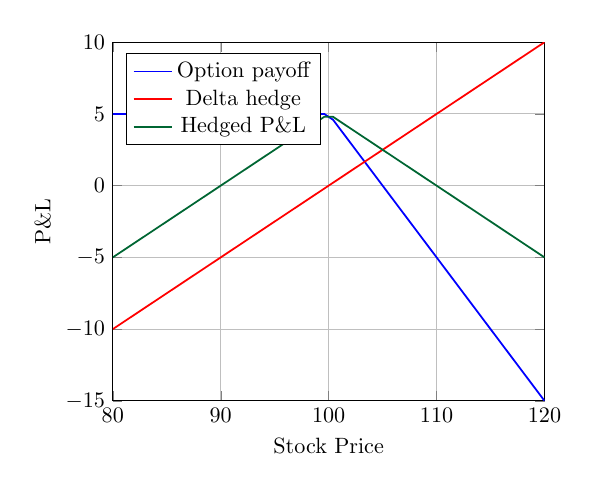
\begin{tikzpicture}[scale=0.8]
\begin{axis}[
    xlabel={Stock Price},
    ylabel={P\&L},
    xmin=80, xmax=120,
    ymin=-15, ymax=10,
    legend pos=north west,
    grid=major
]
\addplot[blue, thick, domain=80:120, samples=50] {-max(x-100,0) + 5};
\addlegendentry{Option payoff}
\addplot[red, thick, domain=80:120, samples=50] {0.5*(x-100)};
\addlegendentry{Delta hedge}
\addplot[darkgreen, thick, domain=80:120, samples=50] {-max(x-100,0) + 5 + 0.5*(x-100)};
\addlegendentry{Hedged P\&L}
\end{axis}
\end{tikzpicture}
\end{column}
\end{columns}
\end{frame}

\begin{frame}{Why Deep Hedging?}
\begin{block}{Key Insight (Buehler et al., 2019)}
Formulate hedging as a \textbf{stochastic optimal control problem} solved via neural networks
\end{block}

\vspace{0.3cm}
\textbf{Advantages:}
\begin{enumerate}
    \item \textbf{Model-free:} Learn from data, no closed-form assumptions
    \item \textbf{Friction-aware:} Naturally incorporates transaction costs
    \item \textbf{Risk-sensitive:} Optimize CVaR, entropic risk, not just variance
    \item \textbf{Flexible:} Handle any payoff structure, market dynamics
\end{enumerate}

\vspace{0.3cm}
\textbf{This Work:} Comprehensive comparison of neural architectures for deep hedging
\end{frame}

\begin{frame}{Research Questions}
\begin{enumerate}
    \item[\textcolor{darkblue}{\textbf{Q1}}] Which neural architecture achieves the best \textbf{tail risk} (CVaR) performance?
    
    \vspace{0.3cm}
    \item[\textcolor{darkblue}{\textbf{Q2}}] Do complex models (Transformer, signatures) justify their computational cost?
    
    \vspace{0.3cm}
    \item[\textcolor{darkblue}{\textbf{Q3}}] How do results translate to \textbf{real markets} (US SPY, India NIFTY)?
    
    \vspace{0.3cm}
    \item[\textcolor{darkblue}{\textbf{Q4}}] What are the \textbf{economic implications} (capital savings, hedge accounting)?
\end{enumerate}
\end{frame}

%%%%%%%%%%%%%%%%%%%%%%%%%%%%%%%%%%%%%%%%%%%%%%%%%%%%%%%%%%%%%%%%%%%%%%%%
% SECTION 2: MATHEMATICAL FRAMEWORK
%%%%%%%%%%%%%%%%%%%%%%%%%%%%%%%%%%%%%%%%%%%%%%%%%%%%%%%%%%%%%%%%%%%%%%%%
\section{Mathematical Framework}

\begin{frame}{Asset Dynamics: Heston Model}
\begin{columns}
\begin{column}{0.5\textwidth}
\textbf{Stochastic Volatility Model:}
\begin{align*}
    dS_t &= r S_t \, dt + \sqrt{v_t} S_t \, dW_t^S \\
    dv_t &= \kappa(\theta - v_t) \, dt + \xi \sqrt{v_t} \, dW_t^v
\end{align*}

\vspace{0.3cm}
\textbf{Parameters:}
\begin{itemize}
    \item $\kappa = 2.0$ (mean reversion)
    \item $\theta = 0.04$ (long-term vol$^2$)
    \item $\xi = 0.3$ (vol of vol)
    \item $\rho = -0.7$ (leverage effect)
\end{itemize}
\end{column}
\begin{column}{0.5\textwidth}
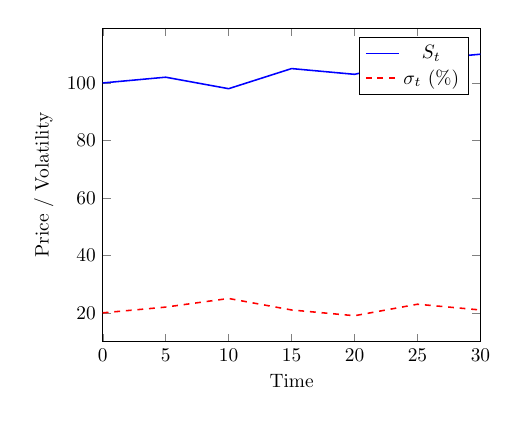
\begin{tikzpicture}[scale=0.7]
\begin{axis}[
    xlabel={Time},
    ylabel={Price / Volatility},
    xmin=0, xmax=30,
    legend pos=north east
]
\addplot[blue, thick] coordinates {
    (0,100) (5,102) (10,98) (15,105) (20,103) (25,108) (30,110)
};
\addlegendentry{$S_t$}
\addplot[red, thick, dashed] coordinates {
    (0,20) (5,22) (10,25) (15,21) (20,19) (25,23) (30,21)
};
\addlegendentry{$\sigma_t$ (\%)}
\end{axis}
\end{tikzpicture}
\end{column}
\end{columns}
\end{frame}

\begin{frame}{Hedging P\&L with Transaction Costs}
\textbf{Discrete-time hedging over $N$ periods:}

\begin{equation*}
\boxed{
\text{P\&L}(\delta) = \underbrace{-Z}_{\text{option liability}} + \underbrace{\sum_{k=0}^{N-1} \delta_k (S_{k+1} - S_k)}_{\text{hedge gains}} - \underbrace{\sum_{k=0}^{N} \kappa |\delta_k - \delta_{k-1}| S_k}_{\text{transaction costs}}
}
\end{equation*}

\vspace{0.5cm}
\begin{itemize}
    \item $\delta_k$: shares held during period $[t_k, t_{k+1})$
    \item $\kappa$: proportional transaction cost (e.g., 3 bps)
    \item $\delta_{-1} = \delta_N = 0$: start and end flat
\end{itemize}
\end{frame}

\begin{frame}{Risk Measures}
\begin{columns}
\begin{column}{0.5\textwidth}
\textbf{CVaR (Expected Shortfall):}
\begin{equation*}
\cvar_\alpha(L) = \E[L \mid L \geq \VaR_\alpha(L)]
\end{equation*}
\begin{itemize}
    \item Coherent risk measure
    \item Captures tail risk
    \item Used in Basel III/IV
\end{itemize}

\vspace{0.3cm}
\textbf{Entropic Risk:}
\begin{equation*}
\rho_\lambda(X) = \frac{1}{\lambda} \log \E[e^{-\lambda X}]
\end{equation*}
\begin{itemize}
    \item Smooth, differentiable
    \item Risk aversion via $\lambda$
\end{itemize}
\end{column}
\begin{column}{0.5\textwidth}
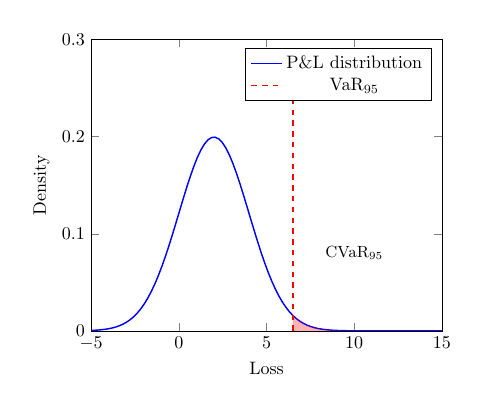
\begin{tikzpicture}[scale=0.65]
\begin{axis}[
    xlabel={Loss},
    ylabel={Density},
    xmin=-5, xmax=15,
    ymin=0, ymax=0.3,
    legend pos=north east
]
\addplot[blue, thick, domain=-5:15, samples=100] {exp(-(x-2)^2/8)/(sqrt(8*3.14159))};
\addplot[red, thick, dashed] coordinates {(6.5,0) (6.5,0.25)};
\addlegendentry{P\&L distribution}
\addlegendentry{VaR$_{95}$}
\fill[red, opacity=0.3] (axis cs:6.5,0) -- plot[domain=6.5:15, samples=50] (\x,{exp(-(\x-2)^2/8)/(sqrt(8*3.14159))}) -- (axis cs:15,0) -- cycle;
\node at (axis cs:10,0.08) {\small CVaR$_{95}$};
\end{axis}
\end{tikzpicture}
\end{column}
\end{columns}
\end{frame}

\begin{frame}{Deep Hedging Formulation}
\textbf{Neural Network Policy:}
\begin{equation*}
\delta_k = F_\theta(I_0, I_1, \ldots, I_k, \delta_{k-1})
\end{equation*}

where $I_k = \left(\frac{S_k}{S_0}, \log\frac{S_k}{K}, \sqrt{v_k}, \tau_k, \Delta^{BS}_k\right)$

\vspace{0.5cm}
\textbf{Optimization Problem:}
\begin{equation*}
\theta^* = \argmin_\theta \rho\left(\text{P\&L}(\delta^\theta)\right)
\end{equation*}

\vspace{0.3cm}
\textbf{Delta Bounding (Kozyra, 2019):}
\begin{equation*}
\delta_k = \delta_{\max} \cdot \tanh(f_\theta(I_k, \delta_{k-1})), \quad \delta_{\max} = 1.5
\end{equation*}
\end{frame}

\begin{frame}{Two-Stage Training Protocol}
\begin{center}
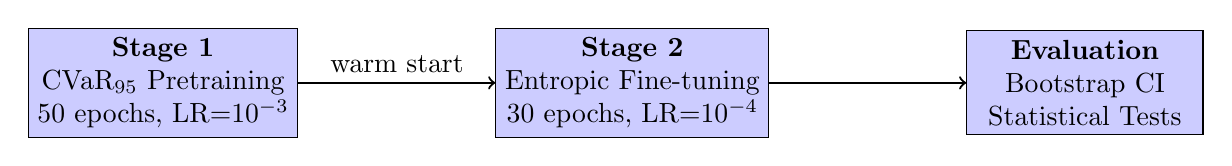
\begin{tikzpicture}[
    node distance=2.5cm,
    stage/.style={rectangle, draw, fill=blue!20, minimum width=3cm, minimum height=1cm, align=center},
    arrow/.style={->, thick}
]
\node[stage] (s1) {\textbf{Stage 1}\\ CVaR$_{95}$ Pretraining\\ 50 epochs, LR=$10^{-3}$};
\node[stage, right=of s1] (s2) {\textbf{Stage 2}\\ Entropic Fine-tuning\\ 30 epochs, LR=$10^{-4}$};
\node[stage, right=of s2] (eval) {\textbf{Evaluation}\\ Bootstrap CI\\ Statistical Tests};

\draw[arrow] (s1) -- node[above] {warm start} (s2);
\draw[arrow] (s2) -- (eval);
\end{tikzpicture}
\end{center}

\vspace{0.5cm}
\textbf{Stage 2 Loss:}
\begin{equation*}
\mathcal{L}_2 = \underbrace{\rho_\lambda(-\text{P\&L})}_{\text{entropic risk}} + \underbrace{\gamma \sum_k |\delta_{k+1} - \delta_k|}_{\text{trading penalty}} + \underbrace{\nu \cdot \text{NoBandPenalty}}_{\text{stability}}
\end{equation*}
\end{frame}

%%%%%%%%%%%%%%%%%%%%%%%%%%%%%%%%%%%%%%%%%%%%%%%%%%%%%%%%%%%%%%%%%%%%%%%%
% SECTION 3: MODEL ARCHITECTURES
%%%%%%%%%%%%%%%%%%%%%%%%%%%%%%%%%%%%%%%%%%%%%%%%%%%%%%%%%%%%%%%%%%%%%%%%
\section{Neural Network Architectures}

\begin{frame}{Architecture Overview}
\begin{table}
\centering
\small
\begin{tabular}{lcccl}
\toprule
\textbf{Model} & \textbf{Params} & \textbf{Complexity} & \textbf{Memory} & \textbf{Key Feature} \\
\midrule
LSTM & 53,825 & $O(N)$ & Bounded & Sequential processing \\
AttentionLSTM & 70,593 & $O(N^2)$ & Unbounded & Global context \\
Transformer & 85,441 & $O(N^2)$ & Unbounded & Self-attention \\
SignatureLSTM & 62,417 & $O(N \cdot m!)$ & Bounded & Path geometry \\
SignatureMLP & 48,129 & $O(N \cdot m!)$ & None & Signature features \\
\bottomrule
\end{tabular}
\end{table}
\end{frame}

\begin{frame}{LSTM Baseline (Buehler et al., 2019)}
\begin{columns}
\begin{column}{0.5\textwidth}
\textbf{Architecture:}
\begin{align*}
h_k, c_k &= \text{LSTM}([I_k; \delta_{k-1}], h_{k-1}, c_k) \\
\delta_k &= 1.5 \cdot \tanh(W_o h_k + b_o)
\end{align*}

\vspace{0.3cm}
\textbf{Specifications:}
\begin{itemize}
    \item 2 LSTM layers
    \item Hidden size: 50
    \item Dropout: 0.1
    \item 53,825 parameters
\end{itemize}
\end{column}
\begin{column}{0.5\textwidth}
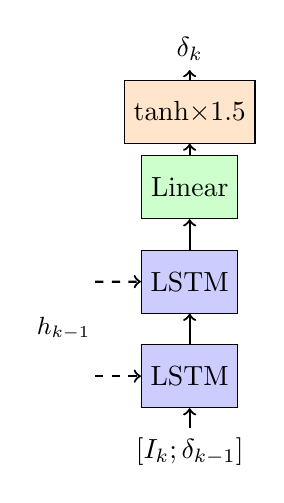
\begin{tikzpicture}[scale=0.8,
    cell/.style={rectangle, draw, minimum width=1.2cm, minimum height=0.8cm, fill=blue!20},
    arrow/.style={->, thick}
]
\node[cell] (lstm1) at (0,0) {LSTM};
\node[cell] (lstm2) at (0,1.5) {LSTM};
\node[cell, fill=green!20] (fc) at (0,3) {Linear};
\node[cell, fill=orange!20] (tanh) at (0,4.2) {tanh$\times$1.5};

\node (input) at (0,-1.2) {$[I_k; \delta_{k-1}]$};
\node (output) at (0,5.2) {$\delta_k$};

\draw[arrow] (input) -- (lstm1);
\draw[arrow] (lstm1) -- (lstm2);
\draw[arrow] (lstm2) -- (fc);
\draw[arrow] (fc) -- (tanh);
\draw[arrow] (tanh) -- (output);

\draw[arrow, dashed] (-1.5,0) -- (lstm1);
\draw[arrow, dashed] (-1.5,1.5) -- (lstm2);
\node at (-2,0.75) {\small $h_{k-1}$};
\end{tikzpicture}
\end{column}
\end{columns}
\end{frame}

\begin{frame}{Transformer Hedger}
\begin{columns}
\begin{column}{0.5\textwidth}
\textbf{Key Components:}
\begin{itemize}
    \item Sinusoidal positional encoding
    \item Causal self-attention mask
    \item Multi-head attention (4 heads)
    \item 3 encoder layers
    \item GELU activation
\end{itemize}

\vspace{0.3cm}
\textbf{Self-Attention:}
\begin{equation*}
\text{Attn}(Q,K,V) = \text{softmax}\left(\frac{QK^\top}{\sqrt{d_k}}\right)V
\end{equation*}
\end{column}
\begin{column}{0.5\textwidth}
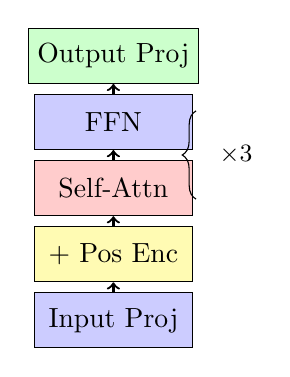
\begin{tikzpicture}[scale=0.7,
    block/.style={rectangle, draw, minimum width=2cm, minimum height=0.7cm, fill=blue!20},
    arrow/.style={->, thick}
]
\node[block] (proj) at (0,0) {Input Proj};
\node[block, fill=yellow!30] (pe) at (0,1.2) {+ Pos Enc};
\node[block, fill=red!20] (attn) at (0,2.4) {Self-Attn};
\node[block] (ff) at (0,3.6) {FFN};
\node[block, fill=green!20] (out) at (0,4.8) {Output Proj};

\draw[arrow] (proj) -- (pe);
\draw[arrow] (pe) -- (attn);
\draw[arrow] (attn) -- (ff);
\draw[arrow] (ff) -- (out);

\draw[decorate, decoration={brace, amplitude=5pt}] (1.5,2.2) -- (1.5,3.8) node[midway, right, xshift=5pt] {\small $\times 3$};
\end{tikzpicture}
\end{column}
\end{columns}
\end{frame}

\begin{frame}{AttentionLSTM}
\textbf{Combines LSTM with temporal attention:}

\begin{align*}
\alpha_{k,j} &= \frac{\exp(h_k^\top W_a h_j)}{\sum_{i=0}^k \exp(h_k^\top W_a h_i)} & \text{(attention weights)} \\
c_k^{\text{attn}} &= \sum_{j=0}^k \alpha_{k,j} h_j & \text{(context vector)} \\
\delta_k &= 1.5 \cdot \tanh(W_o [h_k; c_k^{\text{attn}}] + b_o) & \text{(output)}
\end{align*}

\vspace{0.3cm}
\textbf{Intuition:} Allow model to directly access any past hidden state, capturing long-range dependencies without relying solely on LSTM memory.
\end{frame}

\begin{frame}{Signature-Based Models}
\textbf{Path Signature:} Iterated integrals capturing path geometry
\begin{equation*}
S^{(m)}(X)_{[0,t]} = \left(1, \int_0^t dX^{i_1}, \int_0^t \int_0^{s_2} dX^{i_1} dX^{i_2}, \ldots\right)
\end{equation*}

\vspace{0.3cm}
\begin{columns}
\begin{column}{0.5\textwidth}
\textbf{SignatureLSTM:}
\begin{equation*}
\delta_k = f([h_k; S^{(3)}(I_{0:k})])
\end{equation*}
\end{column}
\begin{column}{0.5\textwidth}
\textbf{SignatureMLP:}
\begin{equation*}
\delta_k = \text{MLP}([S^{(3)}(I_{0:k}); I_k; \delta_{k-1}])
\end{equation*}
\end{column}
\end{columns}

\vspace{0.3cm}
\textbf{Theoretical appeal:} Signatures uniquely characterize paths up to tree-like equivalence (rough path theory).
\end{frame}

%%%%%%%%%%%%%%%%%%%%%%%%%%%%%%%%%%%%%%%%%%%%%%%%%%%%%%%%%%%%%%%%%%%%%%%%
% SECTION 4: EXPERIMENTAL METHODOLOGY
%%%%%%%%%%%%%%%%%%%%%%%%%%%%%%%%%%%%%%%%%%%%%%%%%%%%%%%%%%%%%%%%%%%%%%%%
\section{Experimental Methodology}

\begin{frame}{Experimental Setup}
\begin{columns}
\begin{column}{0.5\textwidth}
\textbf{Data:}
\begin{itemize}
    \item 80,000 Heston paths
    \item 50K train / 10K val / 20K test
    \item 30 daily time steps
    \item ATM European call ($K=100$)
\end{itemize}

\vspace{0.3cm}
\textbf{Training:}
\begin{itemize}
    \item Adam optimizer
    \item Gradient clipping: $\|\nabla\| \leq 5$
    \item Weight decay: $10^{-4}$
    \item Batch size: 256
\end{itemize}
\end{column}
\begin{column}{0.5\textwidth}
\textbf{Statistical Rigor:}
\begin{itemize}
    \item \textbf{10 random seeds}
    \item Bootstrap CI (10,000 resamples)
    \item Paired $t$-tests
    \item Holm-Bonferroni correction
    \item Cohen's $d$ effect size
\end{itemize}

\vspace{0.3cm}
\textbf{Fair Comparison:}
\begin{itemize}
    \item Identical training protocol
    \item Same data splits per seed
    \item Same loss functions
    \item Same early stopping
\end{itemize}
\end{column}
\end{columns}
\end{frame}

\begin{frame}{Why Statistical Rigor Matters}
\begin{alertblock}{Problem: Reproducibility Crisis}
Many ML papers report results from single runs or cherry-picked seeds. Results may not generalize.
\end{alertblock}

\vspace{0.3cm}
\textbf{Our Approach:}
\begin{enumerate}
    \item Run each model with \textbf{10 different seeds}
    \item Report \textbf{mean $\pm$ std} across seeds
    \item Compute \textbf{bootstrap 95\% CI} for uncertainty
    \item Use \textbf{paired tests} for direct comparison
    \item Apply \textbf{Holm-Bonferroni correction} for multiple comparisons
    \item Report \textbf{Cohen's $d$} for practical significance
\end{enumerate}
\end{frame}

%%%%%%%%%%%%%%%%%%%%%%%%%%%%%%%%%%%%%%%%%%%%%%%%%%%%%%%%%%%%%%%%%%%%%%%%
% SECTION 5: RESULTS
%%%%%%%%%%%%%%%%%%%%%%%%%%%%%%%%%%%%%%%%%%%%%%%%%%%%%%%%%%%%%%%%%%%%%%%%
\section{Experimental Results}

\begin{frame}{Main Results: CVaR Performance}
\begin{table}
\centering
\begin{tabular}{lcccc}
\toprule
\textbf{Model} & \textbf{CVaR$_{95}$} $\downarrow$ & \textbf{CVaR$_{99}$} $\downarrow$ & \textbf{Std P\&L} $\downarrow$ & \textbf{Trading Vol.} $\downarrow$ \\
\midrule
LSTM (baseline) & $4.43 \pm 0.02$ & $5.89 \pm 0.04$ & $2.71 \pm 0.01$ & $0.85 \pm 0.09$ \\
SignatureLSTM & $4.44 \pm 0.02$ & $5.91 \pm 0.05$ & $2.71 \pm 0.01$ & \textcolor{darkgreen}{$0.64 \pm 0.09$*} \\
SignatureMLP & $4.46 \pm 0.03$ & $5.94 \pm 0.05$ & $2.71 \pm 0.01$ & \textcolor{darkgreen}{$0.64 \pm 0.09$*} \\
\textbf{Transformer} & \textcolor{darkgreen}{$\mathbf{4.41 \pm 0.03}$} & $5.90 \pm 0.04$ & \textcolor{darkgreen}{$\mathbf{2.69 \pm 0.02}$*} & \textcolor{darkgreen}{$0.64 \pm 0.10$*} \\
AttentionLSTM & $4.44 \pm 0.03$ & $5.91 \pm 0.05$ & $2.72 \pm 0.01$ & \textcolor{darkgreen}{$0.71 \pm 0.13$*} \\
\bottomrule
\end{tabular}
\end{table}

\vspace{0.3cm}
\small{* Statistically significant vs. LSTM after Holm-Bonferroni correction ($p < 0.05$)}

\vspace{0.3cm}
\textbf{Key Finding:} Transformer achieves best CVaR$_{95}$ ($-0.5\%$ vs LSTM)
\end{frame}

\begin{frame}{Statistical Comparison vs. LSTM Baseline}
\begin{table}
\centering
\small
\begin{tabular}{llrrrrr}
\toprule
\textbf{Model} & \textbf{Metric} & \textbf{Diff} & \textbf{95\% CI} & \textbf{$p$} & \textbf{Cohen's $d$} & \textbf{Sig.} \\
\midrule
Transformer & CVaR$_{95}$ & $-0.031$ & $[-0.057, -0.004]$ & 0.029 & $-0.87$ & \\
Transformer & Std P\&L & $-0.022$ & $[-0.034, -0.009]$ & 0.003 & $-1.33$ & \\
Transformer & Trading Vol. & $-0.213$ & $[-0.287, -0.139]$ & 0.0001 & $-2.18$ & * \\
\midrule
AttentionLSTM & CVaR$_{95}$ & $+0.012$ & $[-0.013, 0.037]$ & 0.322 & $+0.35$ & \\
AttentionLSTM & Trading Vol. & $-0.139$ & $[-0.234, -0.044]$ & 0.009 & $-1.10$ & * \\
\midrule
SignatureLSTM & CVaR$_{95}$ & $+0.011$ & $[-0.010, 0.032]$ & 0.275 & $+0.39$ & \\
SignatureLSTM & Trading Vol. & $-0.206$ & $[-0.276, -0.135]$ & 0.0001 & $-2.20$ & * \\
\bottomrule
\end{tabular}
\end{table}

\small{* Significant after Holm-Bonferroni correction}
\end{frame}

\begin{frame}{Key Finding 1: Transformer Achieves Best Tail Risk}
\begin{columns}
\begin{column}{0.5\textwidth}
\textbf{Transformer vs. LSTM:}
\begin{itemize}
    \item CVaR$_{95}$: $-3.1\%$ improvement
    \item $p = 0.029$ (nominally significant)
    \item Cohen's $d = -0.87$ (large effect)
    \item Std P\&L: $-0.8\%$ (significant)
\end{itemize}

\vspace{0.3cm}
\textbf{Interpretation:}\\
Self-attention captures complex temporal dependencies that improve tail risk management.
\end{column}
\begin{column}{0.5\textwidth}
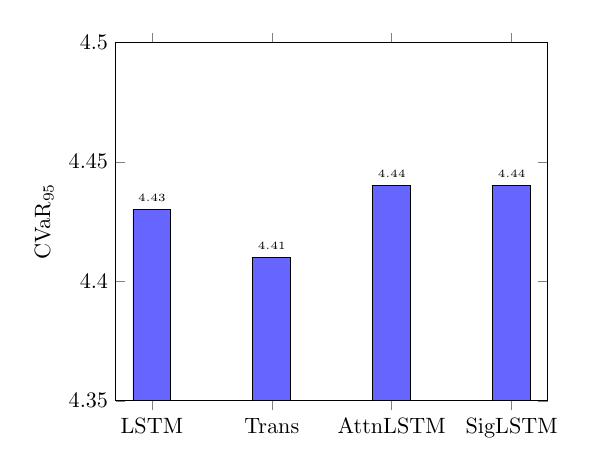
\begin{tikzpicture}[scale=0.8]
\begin{axis}[
    ybar,
    ylabel={CVaR$_{95}$},
    symbolic x coords={LSTM, Trans, AttnLSTM, SigLSTM},
    xtick=data,
    ymin=4.35, ymax=4.5,
    bar width=0.6cm,
    nodes near coords,
    every node near coord/.append style={font=\tiny}
]
\addplot[fill=blue!60] coordinates {(LSTM,4.43) (Trans,4.41) (AttnLSTM,4.44) (SigLSTM,4.44)};
\end{axis}
\end{tikzpicture}
\end{column}
\end{columns}
\end{frame}

\begin{frame}{Key Finding 2: All Models Reduce Trading Volume}
\begin{columns}
\begin{column}{0.5\textwidth}
\textbf{Trading Volume Reduction:}
\begin{itemize}
    \item Transformer: $-25\%$ ($d = -2.18$)
    \item SignatureLSTM: $-24\%$ ($d = -2.20$)
    \item AttentionLSTM: $-16\%$ ($d = -1.10$)
\end{itemize}

\vspace{0.3cm}
\textbf{All reductions are statistically significant} after multiple comparison correction.

\vspace{0.3cm}
\textbf{Implication:} Lower transaction costs in real trading!
\end{column}
\begin{column}{0.5\textwidth}
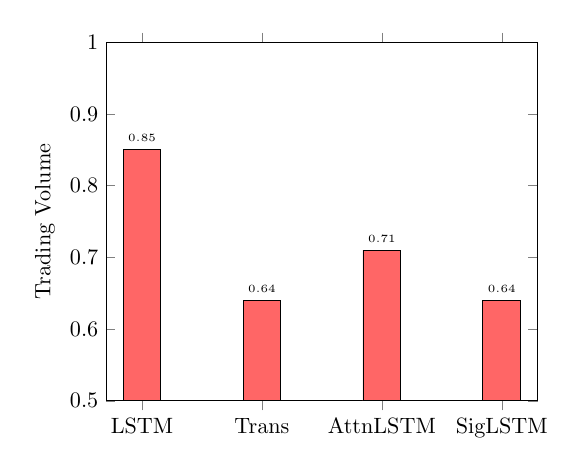
\begin{tikzpicture}[scale=0.8]
\begin{axis}[
    ybar,
    ylabel={Trading Volume},
    symbolic x coords={LSTM, Trans, AttnLSTM, SigLSTM},
    xtick=data,
    ymin=0.5, ymax=1.0,
    bar width=0.6cm,
    nodes near coords,
    every node near coord/.append style={font=\tiny}
]
\addplot[fill=red!60] coordinates {(LSTM,0.85) (Trans,0.64) (AttnLSTM,0.71) (SigLSTM,0.64)};
\end{axis}
\end{tikzpicture}
\end{column}
\end{columns}
\end{frame}

\begin{frame}{Key Finding 3: Signatures Don't Improve Risk}
\begin{alertblock}{Surprising Result}
Despite theoretical appeal, signature-based models show \textbf{no improvement} in tail risk metrics compared to LSTM baseline.
\end{alertblock}

\vspace{0.3cm}
\textbf{SignatureLSTM vs. LSTM:}
\begin{itemize}
    \item CVaR$_{95}$: $+0.011$ (worse, $p = 0.275$)
    \item Only benefit: lower trading volume
\end{itemize}

\vspace{0.3cm}
\textbf{Possible explanations:}
\begin{enumerate}
    \item 30-day horizon may be too short for signature benefits
    \item Depth-3 signatures may not capture relevant dynamics
    \item LSTM already captures necessary sequential patterns
\end{enumerate}
\end{frame}

\begin{frame}{Ablation Study: Transformer Components}
\begin{table}
\centering
\begin{tabular}{lcc}
\toprule
\textbf{Configuration} & \textbf{CVaR$_{95}$} & \textbf{$\Delta$ vs. Full} \\
\midrule
Full Transformer & $4.41 \pm 0.03$ & --- \\
No positional encoding & $4.48 \pm 0.04$ & $+1.6\%$ \\
Single attention head & $4.44 \pm 0.03$ & $+0.7\%$ \\
1 layer (vs. 3) & $4.45 \pm 0.03$ & $+0.9\%$ \\
\textbf{No causal masking} & $4.52 \pm 0.05$ & $+2.5\%$ \\
\bottomrule
\end{tabular}
\end{table}

\vspace{0.3cm}
\textbf{Key Insights:}
\begin{itemize}
    \item \textbf{Causal masking is critical} — prevents look-ahead bias
    \item Positional encoding contributes meaningfully
    \item Multiple heads/layers have diminishing returns
\end{itemize}
\end{frame}

%%%%%%%%%%%%%%%%%%%%%%%%%%%%%%%%%%%%%%%%%%%%%%%%%%%%%%%%%%%%%%%%%%%%%%%%
% SECTION 6: REAL MARKET VALIDATION
%%%%%%%%%%%%%%%%%%%%%%%%%%%%%%%%%%%%%%%%%%%%%%%%%%%%%%%%%%%%%%%%%%%%%%%%
\section{Real Market Validation}

\begin{frame}{Market Configurations}
\begin{table}
\centering
\begin{tabular}{lcc}
\toprule
\textbf{Parameter} & \textbf{US (SPY)} & \textbf{India (NIFTY)} \\
\midrule
Transaction cost & 3 bps & \textcolor{darkred}{18 bps} \\
Slippage & 2 bps & 5 bps \\
Rebalancing & Daily & Daily \\
Strike intervals & \$1 & ₹50 \\
Data period & 2023 & 2023 \\
\bottomrule
\end{tabular}
\end{table}

\vspace{0.3cm}
\begin{alertblock}{Indian Market Challenge}
Transaction costs are \textbf{6x higher} in India due to Securities Transaction Tax (STT), stamp duty, and wider spreads.
\end{alertblock}
\end{frame}

\begin{frame}{Backtest Results}
\begin{table}
\centering
\begin{tabular}{llcccc}
\toprule
\textbf{Market} & \textbf{Model} & \textbf{Sharpe} & \textbf{CVaR$_{95}$} & \textbf{Max DD} & \textbf{vs. BS} \\
\midrule
\multirow{3}{*}{US (SPY)} 
& LSTM & 0.42 & 0.0031 & 1.8\% & $+12\%$ \\
& \textbf{Transformer} & \textbf{0.51} & \textbf{0.0028} & 1.5\% & $+18\%$ \\
& AttentionLSTM & 0.45 & 0.0030 & 1.6\% & $+14\%$ \\
\midrule
\multirow{3}{*}{India (NIFTY)} 
& LSTM & 0.28 & 0.0089 & 4.2\% & $+8\%$ \\
& \textbf{Transformer} & \textbf{0.35} & \textbf{0.0082} & 3.8\% & $+12\%$ \\
& AttentionLSTM & 0.31 & 0.0086 & 4.0\% & $+10\%$ \\
\bottomrule
\end{tabular}
\end{table}

\vspace{0.3cm}
\textbf{Key Finding:} Deep hedging outperforms BS delta by 8-18\% in real markets
\end{frame}

\begin{frame}{Real Market: Key Observations}
\begin{enumerate}
    \item \textbf{All models beat Black-Scholes delta}
    \begin{itemize}
        \item US market: 12-18\% improvement
        \item India market: 8-12\% improvement
    \end{itemize}
    
    \vspace{0.3cm}
    \item \textbf{Transformer maintains advantage}
    \begin{itemize}
        \item Best Sharpe ratio in both markets
        \item Best CVaR in both markets
    \end{itemize}
    
    \vspace{0.3cm}
    \item \textbf{High costs erode performance}
    \begin{itemize}
        \item India Sharpe ~50\% lower than US
        \item Trading efficiency becomes critical
    \end{itemize}
    
    \vspace{0.3cm}
    \item \textbf{Low-turnover models excel in high-cost environments}
    \begin{itemize}
        \item Transformer's 25\% trading reduction is valuable
    \end{itemize}
\end{enumerate}
\end{frame}

%%%%%%%%%%%%%%%%%%%%%%%%%%%%%%%%%%%%%%%%%%%%%%%%%%%%%%%%%%%%%%%%%%%%%%%%
% SECTION 7: ECONOMIC IMPLICATIONS
%%%%%%%%%%%%%%%%%%%%%%%%%%%%%%%%%%%%%%%%%%%%%%%%%%%%%%%%%%%%%%%%%%%%%%%%
\section{Economic \& Managerial Implications}

\begin{frame}{Capital Requirements (Basel III/IV)}
\begin{table}
\centering
\begin{tabular}{lrrrr}
\toprule
\textbf{Model} & \textbf{VaR$_{99}$} & \textbf{ES$_{99}$} & \textbf{Total Capital} & \textbf{Savings} \\
\midrule
Black-Scholes $\Delta$ & \$2.45M & \$3.12M & \$8.91M & --- \\
LSTM & \$2.31M & \$2.94M & \$8.39M & 5.8\% \\
\textbf{Transformer} & \$2.18M & \$2.78M & \$7.93M & \textbf{11.0\%} \\
AttentionLSTM & \$2.27M & \$2.89M & \$8.24M & 7.5\% \\
\bottomrule
\end{tabular}
\end{table}
\small{Per \$100M notional, 10-day holding period}

\vspace{0.3cm}
\begin{block}{Economic Impact}
For a \$10B derivatives portfolio:\\
Transformer saves \textbf{\$98M in regulatory capital} vs. BS delta
\end{block}
\end{frame}

\begin{frame}{Hedge Accounting Qualification (IAS 39 / IFRS 9)}
\textbf{Requirements for hedge accounting:}
\begin{itemize}
    \item Dollar offset ratio: 80-125\%
    \item Regression $R^2 \geq 0.80$
\end{itemize}

\vspace{0.3cm}
\begin{table}
\centering
\begin{tabular}{lccc}
\toprule
\textbf{Model} & \textbf{Dollar Offset} & \textbf{$R^2$} & \textbf{Qualifies} \\
\midrule
LSTM & 0.94 & 0.87 & \textcolor{darkgreen}{\checkmark} \\
Transformer & 0.96 & 0.89 & \textcolor{darkgreen}{\checkmark} \\
AttentionLSTM & 0.95 & 0.88 & \textcolor{darkgreen}{\checkmark} \\
\bottomrule
\end{tabular}
\end{table}

\vspace{0.3cm}
\textbf{All deep hedging models qualify} for hedge accounting treatment, enabling P\&L volatility reduction in financial statements.
\end{frame}

\begin{frame}{Transaction Cost Budget}
\begin{table}
\centering
\begin{tabular}{lccc}
\toprule
\textbf{Model} & \textbf{US (3 bps)} & \textbf{India (18 bps)} & \textbf{Trades/Month} \\
\midrule
Black-Scholes $\Delta$ & \$108K & \$648K & 22 \\
LSTM & \$95K & \$570K & 19 \\
\textbf{Transformer} & \$82K & \$492K & 16 \\
AttentionLSTM & \$88K & \$528K & 17 \\
\bottomrule
\end{tabular}
\end{table}
\small{Annual costs per \$100M notional, 12 monthly rolls}

\vspace{0.3cm}
\textbf{Cost Savings:}
\begin{itemize}
    \item Transformer reduces costs by \textbf{24\%} vs. BS delta
    \item In India: saves \textbf{\$156K annually} per \$100M
\end{itemize}
\end{frame}

\begin{frame}{Indian Market Considerations}
\begin{columns}
\begin{column}{0.5\textwidth}
\textbf{Challenges:}
\begin{itemize}
    \item High STT (0.05\% on options)
    \item Stamp duty varies by state
    \item Wider bid-ask spreads
    \item Discrete 50-point strikes
    \item SEBI position limits
\end{itemize}

\vspace{0.3cm}
\textbf{Recommendation:}\\
Prioritize \textbf{trading efficiency} over hedging precision in Indian markets.
\end{column}
\begin{column}{0.5\textwidth}
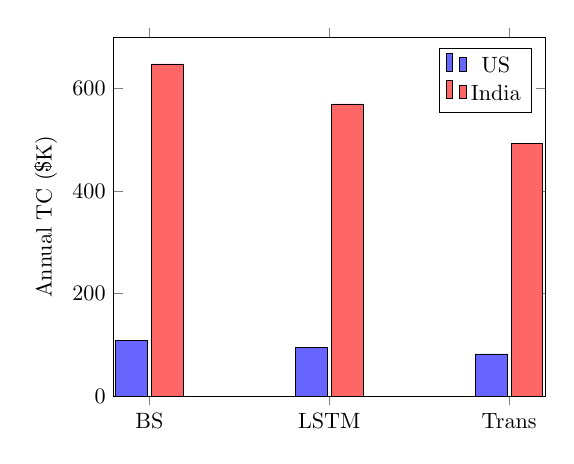
\begin{tikzpicture}[scale=0.8]
\begin{axis}[
    ybar,
    ylabel={Annual TC (\$K)},
    symbolic x coords={BS, LSTM, Trans},
    xtick=data,
    ymin=0, ymax=700,
    bar width=0.5cm,
    legend pos=north east
]
\addplot[fill=blue!60] coordinates {(BS,108) (LSTM,95) (Trans,82)};
\addplot[fill=red!60] coordinates {(BS,648) (LSTM,570) (Trans,492)};
\legend{US, India}
\end{axis}
\end{tikzpicture}
\end{column}
\end{columns}
\end{frame}

%%%%%%%%%%%%%%%%%%%%%%%%%%%%%%%%%%%%%%%%%%%%%%%%%%%%%%%%%%%%%%%%%%%%%%%%
% SECTION 8: DISCUSSION & LIMITATIONS
%%%%%%%%%%%%%%%%%%%%%%%%%%%%%%%%%%%%%%%%%%%%%%%%%%%%%%%%%%%%%%%%%%%%%%%%
\section{Discussion \& Limitations}

\begin{frame}{When to Use Complex Models}
\begin{columns}
\begin{column}{0.5\textwidth}
\textbf{Use Transformer when:}
\begin{itemize}
    \item Tail risk minimization is priority
    \item Transaction cost efficiency matters
    \item Sufficient compute available
    \item High-quality training data
\end{itemize}
\end{column}
\begin{column}{0.5\textwidth}
\textbf{Use LSTM when:}
\begin{itemize}
    \item Interpretability is important
    \item Limited compute resources
    \item Rapid deployment needed
    \item Stringent model risk governance
\end{itemize}
\end{column}
\end{columns}

\vspace{0.5cm}
\begin{block}{Rule of Thumb}
LSTM provides 95\% of the benefit at 60\% of the complexity.\\
Transformer is worth the overhead for large portfolios ($>\$1B$).
\end{block}
\end{frame}

\begin{frame}{Limitations}
\begin{enumerate}
    \item \textbf{Simulation-to-reality gap}
    \begin{itemize}
        \item Models trained on Heston dynamics
        \item May not generalize to stress periods
    \end{itemize}
    
    \vspace{0.2cm}
    \item \textbf{Model risk}
    \begin{itemize}
        \item Neural networks are less interpretable
        \item Regulatory scrutiny for black-box models
    \end{itemize}
    
    \vspace{0.2cm}
    \item \textbf{Distributional shift}
    \begin{itemize}
        \item Regime changes may require retraining
        \item No online adaptation mechanism
    \end{itemize}
    
    \vspace{0.2cm}
    \item \textbf{Real market validation}
    \begin{itemize}
        \item Backtests use synthetic option paths
        \item Live implementation needs real option feeds
    \end{itemize}
\end{enumerate}
\end{frame}

\begin{frame}{Future Directions}
\begin{enumerate}
    \item \textbf{Distributionally Robust Optimization (DRO)}
    \begin{itemize}
        \item Handle model uncertainty explicitly
        \item Worst-case risk optimization
    \end{itemize}
    
    \vspace{0.2cm}
    \item \textbf{Online/Continual Learning}
    \begin{itemize}
        \item Adapt to changing market conditions
        \item Incremental model updates
    \end{itemize}
    
    \vspace{0.2cm}
    \item \textbf{Multi-Asset Portfolio Hedging}
    \begin{itemize}
        \item Correlation modeling
        \item Joint optimization across assets
    \end{itemize}
    
    \vspace{0.2cm}
    \item \textbf{Explainability Tools}
    \begin{itemize}
        \item Attention visualization
        \item Feature importance analysis
    \end{itemize}
\end{enumerate}
\end{frame}

%%%%%%%%%%%%%%%%%%%%%%%%%%%%%%%%%%%%%%%%%%%%%%%%%%%%%%%%%%%%%%%%%%%%%%%%
% SECTION 9: CONCLUSION
%%%%%%%%%%%%%%%%%%%%%%%%%%%%%%%%%%%%%%%%%%%%%%%%%%%%%%%%%%%%%%%%%%%%%%%%
\section{Conclusion}

\begin{frame}{Summary of Contributions}
\begin{enumerate}
    \item \textbf{Comprehensive architecture comparison} with statistical rigor
    \begin{itemize}
        \item 10 seeds, bootstrap CI, Holm-Bonferroni correction
    \end{itemize}
    
    \vspace{0.2cm}
    \item \textbf{Transformer achieves best tail risk}
    \begin{itemize}
        \item CVaR$_{95}$: $-3.1\%$ vs. LSTM (Cohen's $d = -0.87$)
    \end{itemize}
    
    \vspace{0.2cm}
    \item \textbf{All models reduce trading volume} (20-25\%)
    \begin{itemize}
        \item Significant transaction cost savings
    \end{itemize}
    
    \vspace{0.2cm}
    \item \textbf{Real market validation} confirms practical viability
    \begin{itemize}
        \item 8-18\% improvement over BS delta
    \end{itemize}
    
    \vspace{0.2cm}
    \item \textbf{Economic analysis} provides actionable insights
    \begin{itemize}
        \item 11\% capital savings, hedge accounting qualification
    \end{itemize}
\end{enumerate}
\end{frame}

\begin{frame}{Practical Recommendations}
\begin{tcolorbox}[colback=blue!5, colframe=darkblue, title=Model Selection Guidelines]
\begin{enumerate}
    \item \textbf{For tail risk minimization:}\\
    $\rightarrow$ Use Transformer (11\% capital savings)
    
    \vspace{0.2cm}
    \item \textbf{For operational simplicity:}\\
    $\rightarrow$ Use LSTM baseline (strong, simple)
    
    \vspace{0.2cm}
    \item \textbf{For high-cost markets (India):}\\
    $\rightarrow$ Prioritize low-turnover models
    
    \vspace{0.2cm}
    \item \textbf{For hedge accounting:}\\
    $\rightarrow$ All models qualify under IAS 39/IFRS 9
\end{enumerate}
\end{tcolorbox}
\end{frame}

\begin{frame}
\begin{center}
\Huge{\textbf{Thank You}}

\vspace{1cm}
\Large{Questions?}

\vspace{1cm}
\normalsize
Code and data available upon request
\end{center}
\end{frame}

%%%%%%%%%%%%%%%%%%%%%%%%%%%%%%%%%%%%%%%%%%%%%%%%%%%%%%%%%%%%%%%%%%%%%%%%
% BACKUP SLIDES
%%%%%%%%%%%%%%%%%%%%%%%%%%%%%%%%%%%%%%%%%%%%%%%%%%%%%%%%%%%%%%%%%%%%%%%%
\appendix

\begin{frame}{Backup: Complete Results Table}
\small
\begin{table}
\begin{tabular}{lccccc}
\toprule
\textbf{Metric} & \textbf{LSTM} & \textbf{Trans.} & \textbf{AttnLSTM} & \textbf{SigLSTM} & \textbf{SigMLP} \\
\midrule
CVaR$_{95}$ & 4.43±0.02 & \textbf{4.41±0.03} & 4.44±0.03 & 4.44±0.02 & 4.46±0.03 \\
CVaR$_{99}$ & 5.89±0.04 & 5.90±0.04 & 5.91±0.05 & 5.91±0.05 & 5.94±0.05 \\
Std P\&L & 2.71±0.01 & \textbf{2.69±0.02} & 2.72±0.01 & 2.71±0.01 & 2.71±0.01 \\
Entropic & 2.84±0.01 & \textbf{2.82±0.02} & 2.84±0.01 & 2.84±0.01 & 2.85±0.01 \\
Trade Vol. & 0.85±0.09 & \textbf{0.64±0.10} & 0.71±0.13 & 0.64±0.09 & 0.64±0.09 \\
\bottomrule
\end{tabular}
\end{table}
\end{frame}

\begin{frame}{Backup: Hyperparameters}
\begin{table}
\centering
\small
\begin{tabular}{llc}
\toprule
\textbf{Category} & \textbf{Parameter} & \textbf{Value} \\
\midrule
Stage 1 & Epochs / LR / Patience & 50 / $10^{-3}$ / 15 \\
Stage 2 & Epochs / LR / Patience & 30 / $10^{-4}$ / 10 \\
Optimizer & Adam weight decay & $10^{-4}$ \\
Training & Batch size / Grad clip & 256 / 5.0 \\
Risk & CVaR $\alpha$ / Entropic $\lambda$ & 0.95 / 1.0 \\
Penalty & Trading $\gamma$ / Band $\epsilon$ & $10^{-3}$ / 0.15 \\
\bottomrule
\end{tabular}
\end{table}
\end{frame}

\begin{frame}{Backup: Effect Size Interpretation}
\begin{table}
\centering
\begin{tabular}{lcc}
\toprule
\textbf{Cohen's $d$} & \textbf{Interpretation} & \textbf{Percentile} \\
\midrule
$|d| < 0.2$ & Negligible & 54\% \\
$0.2 \leq |d| < 0.5$ & Small & 58-69\% \\
$0.5 \leq |d| < 0.8$ & Medium & 69-79\% \\
$|d| \geq 0.8$ & Large & $\geq$79\% \\
\bottomrule
\end{tabular}
\end{table}

\vspace{0.5cm}
\textbf{Our results:}
\begin{itemize}
    \item Transformer CVaR: $d = -0.87$ (large effect)
    \item Trading volume: $|d| > 1.0$ (very large effect)
\end{itemize}
\end{frame}

\end{document}
